\documentclass[article]{IEEEtran}

\usepackage{cite}
\usepackage{amsmath,amssymb,amsfonts}
\usepackage{algorithmic}
\usepackage{graphicx}
\usepackage{textcomp}
\usepackage{xcolor}
\usepackage{flushend}
\usepackage{listings}

\usepackage[utf8]{inputenc}
\def\BibTeX{{\rm B\kern-.05em{\sc i\kern-.025em b}\kern-.08em
    T\kern-.1667em\lower.7ex\hbox{E}\kern-.125emX}}
\begin{document}

\title{Processamento de Streams\\Análise a Corridas de Táxis}


\author{\IEEEauthorblockN{André Lopes - 45617 }\\
\and
\IEEEauthorblockN{Nelson Coquenim - 45694}\\
\IEEEauthorblockA{\textit{Departamento de Informática} \\
\textit{Faculdade de Ciências e Tecnologia da Universidade Nova de Lisboa }\\
Almada, Portugal}
}

\maketitle



\section{Introdução}
Este projecto foi desenvolvido no âmbito da cadeira de Processamento de \textit{Streams} (PStr). O objectivo passa por implementar de novo as \textit{queries} do primeiro projecto de PStr, nomeadamente as do  DEBS Grand Challenges 2015. A diferença é que desta vez serão implementadas usando SiddhiQL do WSO2 no lugar do SparkStreaming. Para além destas, serão implementadas mais 3 \textit{queries} que serão descritas mais à frente.

O WSO2 Complex Event Processor (CEP) ajuda a identificar os eventos e padrões mais significativos vindos de múltiplas \textit{sources}, analisando o seu impacto e agindo em \textit{real-time}. O WSO2 CEP apoia-se numa linguagem designada SiddhiQL, que é fácil de usar devido à sua semelhança ao SQL, sendo esta especializada em \textit{queries} complexas envolvendo janelas e detecção tanto de padrões como de sequências.


A implementação de \textit{queries} semelhantes às do primeiro projecto permitirá uma comparação entre as duas tecnologias em termos de performance, manutenção e flexibilidade. A manutenção será avaliada através da comparação da simplicidade do código, pois será possível fazer o paralelo entre o código das \textit{queries} em SiddhiQL e em SparkStreaming, assinalando os benefícios de utilizar uma linguagem de alto nível. No que toca à flexibilidade, o SiddhiQL oferece uma semântica de sequência que permite a identificação de padrões complexos.

	
	
\section{\textit{Setup}}

A \textit{source} dos eventos processados pelo WSO2 CEP é o Apache Kafka. De forma a executar o Kafka é necessário primeiro executar uma instância do Zookeper que tem como benefício a coordenação dos \textit{brokers} do Kafka, o que neste caso não seria necessário, mas o Kafka tem essa obrigatoriedade.

Tendo o \textit{broker} activo, é necessário executar um produtor Kafka, neste caso implementado em Java, que emite os eventos de corridas de táxis com uma cadência configurável. Este produtor lê de um \textit{dataset}, no qual cada linha corresponde a uma viagem de táxi, e emite para o \textit{broker}. Sendo o Kafka um sistema \textit{topic-based}, o tópico no qual estes eventos são publicados é designado "debs". A cadência de eventos foi definida como sendo 60, o que significa que 1 minuto corresponderá a 1 segundo.

De forma a registar as \textit{queries} SiddhiQL que implementam as interrogações definidas, utilizou-se o Stream Processor Studio do WSO2. Este permite, entre outros, instalar \textit{queries} e definir os adaptadores necessários, que permitem consumir a \textit{stream} de eventos através do \textit{broker} Kafka. Para isto, é necessário definir qual o tópico que se pretende subscrever, e como referido anteriormente no caso da produção dos eventos, será o "debs".

A cada evento que chega ao CEP \textit{engine} serão executadas as \textit{queries} instaladas, resultando destas novas \textit{streams}. Por este motivo é importante definir um conjunto de \textit{sinks}, para as quais serão emitidos os novos eventos produzidos pelo processamento dos eventos emitidos pelas \textit{sources}. Nesta implementação foi definido que a \textit{sink} é o \textit{broker} do Kafka, sendo que para cada \textit{query} existirá um produtor de eventos com um tópico diferente. Esta implementação permitirá que qualquer aplicação subscreva a \textit{stream} de \textit{output} que desejar, tendo os dados processados em \textit{real-time}.
 





\section{\textit{Queries}}
Para cada \textit{query} será apresentada a sua descrição, a sua implementação acompanhada de uma explicação e os seus resultados.

\subsection{\textit{Frequent Routes}}

O objectivo desta primeira \textit{query} é achar o \textit{top} 10 das rotas mais frequentes durante um período de 30 minutos. Um rota é representada por uma \textit{cell} inicial e uma \textit{cell} final.

Na Figura \ref{fig:frequentRoutesDiagram} pode se observar a estrutura desta query. Primeiramente efetua-se uma janela deslizante de 30 minutos sobre o input. Finalmente, seleciona-se os 10 resultados com a frequência mais alta.

\begin{figure}[hbtp]
    \centering
        
\includegraphics[width=0.4\textwidth]{images/frequentRoutesDiagram}
    \caption{Diagrama da query \textit{Frequent Routes}.}
    \label{fig:frequentRoutesDiagram}
\end{figure}

O código siddhi que implementa esta \textit{query} é o seguinte:

\begin{lstlisting}[language=SQL]
from TaxiSecStr#window.time(30 minutes)
select pickup_gridID,
  dropoff_gridID,
  count(*) as frequency
group by pickup_gridID,
  dropoff_gridID
order by frequency DESC
insert into RouteFrequencyStr;

from RouteFrequencyStr#window.length(10)
select *
insert into TopFreqRoutesStr;
\end{lstlisting}

\subsection{\textit{Profitables Areas}}

Nesta query pretende-se identificar, de forma contínua, as áreas que são mais lucrativas para os taxistas. Para tal, o lucro de uma área é definido pelas receitas geradas nessa área a dividir pelo número de táxis vazios nessa mesma área.

A receita gerada numa área é a média das \textit{fare} + \textit{tip} de todas as corridas que originaram nessa área e que acabaram nos 15 minutos seguintes.

O número de táxis vazios num dada área consiste na soma dos táxis que efetuaram uma \textit{dropoff} nessa área mas que após 30 minutos ainda não efetuaram uma \textit{pickup}.

Na Figura \ref{fig:profitablesAreasDiagram} pode-se observar um diagrama que demonstra o fluxo desta \textit{query}.

\begin{figure}[hbtp]
    \centering
        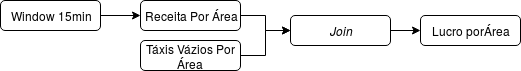
\includegraphics[width=0.4\textwidth]{images/profitableAreasDiagram_v3}
    \caption{Diagrama da query \textit{Profitables Areas}.}
    \label{fig:profitablesAreasDiagram}
\end{figure}

O código siddhi que implementa esta \textit{query} é o seguinte:

\begin{lstlisting}[language=SQL]
from TaxiSecStr#window.time(15 min)
select pickup_gridID as areaID
   avg(FareTrip) as revenue
group by pickup_gridID
insert into RevenuePerAreaStr;

from e1 = TaxiSecStr ->
  TaxiSecStr[medallion==e1.medallion 
  and pickup_datetime 
  - e1.dropoff_datetime>30 mins]
select dropoff_gridID as areaID
insert into EmptyTaxisAreasStr;

partition with 
   (areaID of RevenuePerAreaStr)
begin
  from EmptyTaxisAreasStr
  select areaID, count(*) as emptyTaxis
  insert into #EmptyTaxisPerAreaStr;

  from RevenuePerAreaStr as A 
            join
  #EmptyTaxisPerAreaStr as B 
    on A.areaID == B.areaID
  select A.areaID,
    revenue/emptyTaxis as profit
  insert into ProfitPerAreaStr;
end;
\end{lstlisting}

\subsection{\textit{Idle Taxis}}

Neste \textit{use case} espera-se que seja emitido um alerta quando o número de táxis disponíveis torna-se superior ao pretendido. Para tal, deverá ser publicado um aviso quando o tempo de paragem médio (\textit{idle time}) de todos os táxis é superior a 10 minutos. Define-se como tempo de paragem, o período de tempo entre uma \textit{dropoff} e uma \textit{pickup}. Finalmente, assume-se que um táxi encontra-se disponível se tiver realizado pelo menos uma viagem na última hora.

O diagrama na Figura \ref{fig:idleTaxisDiagram} demonstra a lógica da implementação desta \textit{query}.

\begin{figure}[hbtp]
    \centering
        
\includegraphics[width=0.4\textwidth]{images/idleTaxisDiagram}
    \caption{Diagrama da query \textit{Idle Taxis}.}
    \label{fig:idleTaxisDiagram}
\end{figure}

Em seguida, apresenta-se o excerto de código da \textit{query} em questão:
\begin{lstlisting}[language=SQL]
from TaxiSecStr#window.time(1 hour)
select *
insert into AvailableTaxisStr;

from e1 = AvailableTaxisStr -> 
  e2 = AvailableTaxisStr[medallion
    == e1.medallion]
select e1.medallion as taxi,
  (e2.p_time-e1.d_time) as idle_time
insert into IdleTimeTaxisStr;

from IdleTimeTaxisStr
select avg(idle_time) as avg_idle_time
having avg_idle_time > 10 * 60
insert into IdleTaxisStr;
\end{lstlisting}


\subsection{\textit{Congested Areas}}

Nesta secção ir-se-à implementar uma \textit{query} que emita as localizações onde possivelmente poderá haver congestionamentos no trânsito. Para tal, dever-se-á detetar picos nas durações das viagens dos táxis que são seguidos por pelo menos 3 viagens todas estas com durações crescentes.

A Figura \ref{fig:congestedAreasDiagram} expõe o racional na construção desta \textit{query}.

\begin{figure}[hbtp]
    \centering
        
\includegraphics[width=0.4\textwidth]{images/congestedAreas}
    \caption{Diagrama da query \textit{Congested Areas}.}
    \label{fig:congestedAreasDiagram}
\end{figure}

Finalmente, apresenta-se o código siddhi da \textit{query} \textit{congested areas}:

\begin{lstlisting}[language=SQL]
from every e1 = TaxiSecStr ->
  e2 = TaxiSecStr[medallion==e1.medallion
  and ride_duration > e1.ride_duration] ->
  e3 = TaxiSecStr[medallion==e2.medallion
  and ride_duration < e2.ride_duration] ->
  e4 = TaxiSecStr[medallion==e3.medallion
  and ride_duration > e3.ride_duration] ->
  e5 = TaxiSecStr[medallion==e4.medallion
  and ride_duration > e4.ride_duration] ->
  e6 = TaxiSecStr[medallion==e5.medallion
  and ride_duration > e5.ride_duration]
select e2.pickup_grid_x as grid_x,
  e2.pickup_grid_y as grid_y
insert into CongestedAreasStr;
\end{lstlisting}



\subsection{\textit{Most Pleasant Taxi Drivers}}

Para recompensar os condutores de táxis mais simpáticos é necessário que seja emitido, uma vez por dia, o taxista que recebeu mais gorjetas nesse dia.

O fluxo da Figura \ref{fig:pleasantDriverDiagram} demonstra a construção desta \textit{query}.

\begin{figure}[hbtp]
    \centering
    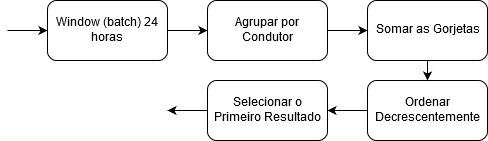
\includegraphics[width=0.4\textwidth]{images/pleasantDriver}
    \caption{Diagrama da query \textit{Most Pleasant Taxi Driver}.}
    \label{fig:pleasantDriverDiagram}
\end{figure}



Por último, no segmento de código seguinte apresenta-se a solução referente a este \textit{use case}:

\begin{lstlisting}[language=SQL]
from TaxiSecStr#window.timeBatch(24 hour)
select driver, 
  sum(tip_amount) as tips_total
group by driver
order by tips_total DESC
insert into TodayDriversTips;

from TodayDriversTips#window.length(1)
select *
insert into PleasantDriverStr;
\end{lstlisting}

\section{\textit{Dashboard}} 
		Apresentação geral
		
		E detalhe do setup e implementação 
		
\section{\textit{Performance comparison}} 
comparar com primeiro trabalho
		
\section{Conclusão} 
-manutenção e flexibilidade vs performance

-documentação reduzida

-detalhes de implementação seriam importantes para entender como funcionam as janelas. Será como no CQL? Não há muita informação disponível. Resulta numa dificuldade de saber onde pôr as janelas

-stream processor studio, o editor é bastante mau devido a quão vago são os erros que dá

-Linguagem alto nível bastante mais expressiva




\bibliography{bibliography}

\bibliographystyle{IEEEtran}
\end{document}
